\clearpage
\phantomsection

\setcounter{chapter}{0}
\chapter[{CƠ SỞ LÝ THUYẾT}]{Cơ sở lý thuyết}
\section{Đặt vấn đề}
Sự phát triển mạnh mẽ của AI trong nhiều năm trở lại đây đã thúc đẩy mạnh mẽ tới sự phát triển của nhiều ngành nghề. Các ứng dụng và giải pháp AI xuất hiện ngày càng phổ biến trong nhiễu lĩnh vực bao gồm tài chính, chăm sóc sức khỏe, bảo mật, ... Năm 2022, thị trường AI toàn cầu được định giá khoảng 454.12 tỷ USD và dự kiến đạt 2575.16 tỷ USD vào năm 2032 \cite{AIMARKET}. Theo khảo sát của McKinsey, tỷ lệ doanh nghiệp áp dụng AI ít nhất trong một chức năng đã tăng từ 20\% năm 2017 lên 50\% năm 2022 \cite{mckinsey}.

Với sự phát triển mạnh mẽ đó, các nhu cầu về việc tăng tốc AI bằng các phần cứng chuyên biệt cũng được tăng theo. Thị trường tăng tốc AI toàn cầu đạt khoảng 19.89 tỷ USD và dự kiến tăng trưởng với tốc độ CAGR 29.4\% từ 2024 đến 2030 \cite{aiaccelerator}. 
Field-Programmable Gate Arrays (FPGAs) là một trong những giải pháp linh hoạt, hiệu quả cho việc triển khai các thiết kế phần cứng tùy chỉnh cho từng ứng dụng AI. Với khả năng tính toán song song mạnh mẽ, ta có thể đạt được hiệu suất cao và độ trễ thấp kể cả đối với các thuật toán xử lý phức tạp. Bên cạnh đó, việc tối ưu hóa năng lượng tiêu thụ và tối ưu hóa I/O có thể đem lại những giá trị có lợi hơn cho nhiều giải pháp. Các nghiên cứu của Apriorit cũng chỉ ra rằng, FPGAs có thể cải thiện hiệu suất tổng thể của các ứng dụng AI \cite{apriorit}.
\section{Trích xuất đặc trưng}
\subsection{Khái niệm trích xuất đặc trưng}
Trích xuất đặc trưng là quá trình chuyển đổi các dữ liệu thô thành các dữ liệu số mà có thể xử lý bởi các mô hình mà vẫn đảm bảo được thông tin từ dữ liệu gốc. Việc trích xuất đặc trưng sẽ đem lại kết quả tốt hơn đối với nhiều thuật toán, giảm chiều và độ phức tạp của dữ liệu. Việc trích xuất đặc trưng có thể bao gồm việc lấy ra các dữ liệu đã có trong dữ liệu gốc hoặc tạo ra các đặc trưng mới bằng các kỹ thuật đặc trưng. Các đặc trưng này có thể coi là đặc tính của một đối tượng dữ liệu. Từ những đặc tính đã được trích xuất, các mô hình có thể đạt được các kết quả tốt hơn trong khi lượng thông tin cần xử lý là ít hơn, đảm bảo được hiệu suất xử lý. 

Trong xử lý ảnh, trích xuất đặc trưng mô tả các thông tin mang tính hình dạng có liên quan trong một mẫu để nhiệm vụ phân loại mẫu có thể thực hiện dễ dàng \cite{featureImgprocessing}. Có thể coi trích xuất đặc trưng là một dạng đặc biệt của giảm chiều dữ liệu. Mục tiêu chính của trích xuất đặc trưng là đạt được các thông tin liên quan của đối tượng từ dữ liệu gốc và biểu diễn chúng ở một chiều dữ liệu nhỏ hơn. Khi mà đầu vào của một thuật toán là quá lớn để xử lý, nó cần được loại bỏ dư thừa. Do đó, dữ liệu cần phải được giảm thiểu bằng cách biểu diễn dưới tập các đặc trưng có ý nghĩa. 
\subsection{Kết cấu thị giác}

\begin{figure} [h]
	\centering
	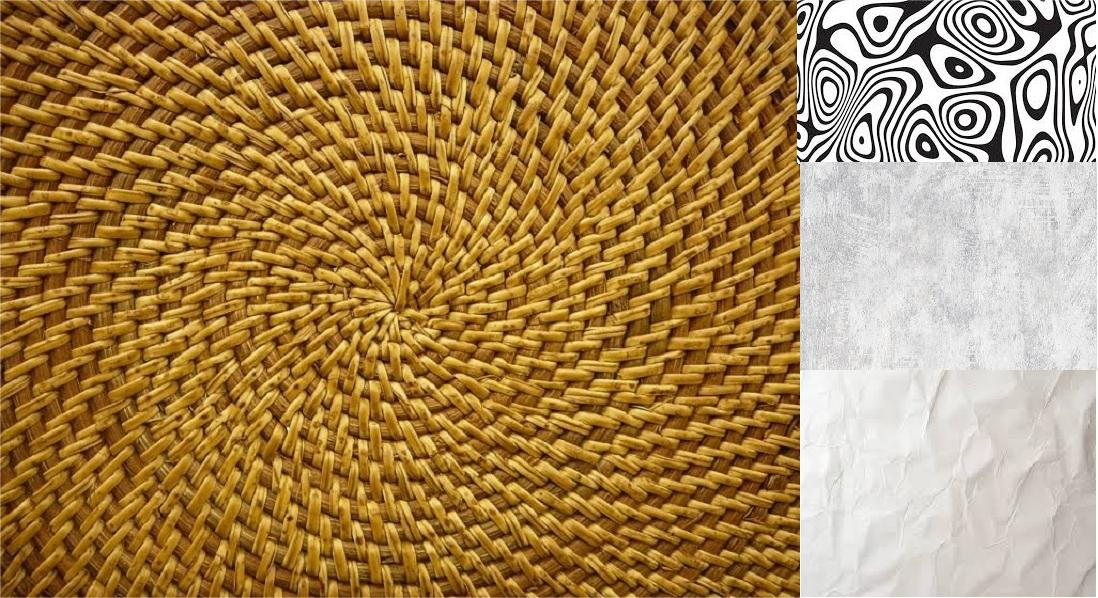
\includegraphics[width=0.8\linewidth]{figures/image1.png}
	\caption{Hình ảnh mẫu về kết cấu}
	\label{fig:image1}
\end{figure}
Texture hay kết cấu bề mặt là một khái niệm cơ bản trong lĩnh vực hình ảnh và thị giác máy tính đề cập đến các đặc điểm cơ bản của hầu hết mọi bề mặt tự nhiên có mặt ở khắp mọi nơi trong hình ảnh tự nhiên. Những đặc điểm này bao gồm kích thước, hình dáng, mật độ, sự sắp xếp và tỷ lệ của các thành phần cơ bản tạo nên thành phần đó. Trong thị giác máy tính, kết cấu đóng vai trò là một trong những đặc điểm quan trọng nhất để nhận diện và phân biệt các đối tượng hoặc các vùng quan tâm trong ảnh. Phân loại kết cấu là bài toán cơ bản được ứng dụng trong nhiều lĩnh vực như chuẩn đoán y khoa \cite{medicalImage}, dầu và gas \cite{textureBasedTechniques}, nông nghiệp \cite{smartFarming}, phân tích hình ảnh y sinh, hình ảnh vệ tinh, ... Mục tiêu chính của phân loại kết cấu là xây dựng một mô hình có khả năng mô tả nội dung kết cấu đã biết dựa trên dữ liệu huấn luyện. Tuy nhiên, để phân biệt được sự khác biệt giữa các kết cấu là vấn đề khá khó khăn vì các kết cấu thực tế thường có nhiều độ phân giải khác nhau, độ quay tùy ý và có thể được chiếu sáng bởi nhiều điện kiện chiếu sáng khác nhau. Điều này yêu cầu các phương pháp cần có khả năng phân tích được tính bất biến của đối tượng.


Một đặc trưng kết cấu tốt được mong đợi bởi đáp ứng 2 yếu tố: Độ phức tạp tính toán thấp cho phép phù hợp với các tác vụ phân loại thời gian thực và nắm bắt được thông tin kết cấu đại diện của một lớp kết cấu, sao cho các lớp kết cấu khác nhau có thể được phân biệt mặc dù có sự hiện diện của nhiều dạng hình ảnh khác nhau (bao gồm độ sáng, độ xoay, tỷ lệ, điểm nhìn, nhiễu, ...).


\subsection{Các phương pháp trích xuất đặc trưng}
Để phân loại kết cấu một cách hiệu quả, cần phải có các phương pháp mô tả và trích xuất đặc trưng của từng loại kết cấu. Có thể chia chúng thành 3 loại bao gồm: phương pháp thống kê, phương pháp mô hình và phương pháp bộ lọc \cite{analyticOfTexture}.

\begin{table}[h]
    \centering
    \renewcommand{\arraystretch}{1.3} % Tăng khoảng cách dòng
        \caption{Các phương pháp trích xuất đặc trưng}
    \begin{tabular}{p{3cm} p{7cm} p{3cm} p{2cm}}
        \toprule
        \textbf{Phương pháp} & \textbf{Đặc điểm} & \textbf{Phân loại} & \textbf{Thuật toán} \\
        \midrule
        Thống kê & Phân tích sự phân bố không gian của các giá trị độ xám trong ảnh bằng cách tính toán các đặc trưng cục bộ, cung cấp các thông tin về độ sáng, độ tương phản, ... & Bậc nhất, bậc 2 và bậc cao& GLCM, LBP, ... \\
        \midrule
        Mô hình & Xây dựng các mô hình toán học để mô tả kết cấu trong ảnh, sau đó trích xuất các tham số của mô hình này thông qua phân tích kết cấu. Bằng cách giả định rằng kết cấu được tạo ra bởi một quá trình ngẫu nhiên hoặc tuân theo một quá trình toán học cụ thể, các tham số của mô hình có thể được sử dụng làm đặc trưng để phân loại & Ngẫu nhiên, fractal, tự hồi quy & MRF, ... \\

                \midrule
        Bộ lọc & Sử dụng các bộ lọc để biến đổi ảnh gốc, sau đó năng lượng của các phản hồi bộ lọc được tính toán tạo thành các đặc trưng kết cấu & Miền không gian, miền tần số, miền không gian - tần số & Gabor filters, Wavelet transforms, ... \\
                        \bottomrule

    \end{tabular}

    \label{tab:texture_analysis}
\end{table}

\newpage
\subsection{Local Binary Pattern}
\label{sec:lbp}
Một vài cách tiếp cận về tính bất biến của độ quay của kết cấu có thể kể đến ảnh cực đồ \cite{polarograms}. Một vài cách khác được đề xuất bằng cách chỉnh sửa các phương pháp đã có như mô hình MRF (Markov Random Field), bộ lọc Gabor hoặc LBP. Trong đó, LBP là một trong những phương pháp thường được sử dụng để mô tả các đặc trưng kết cấu bởi độ phức tạp tính toán thấp, dễ triển khai và bất biến với sự thay đổi ánh sáng đơn điệu \cite{Liu2016}.

Local Binary Pattern (LBP) là một phương pháp thuộc nhóm phương pháp thống kê, được sử dụng để mô tả các mô tả kết cấu (texture descriptors). LBP được giới thiệu lần đầu tiên vào năm 1994 \cite{firstLBP}, có khả năng mô tả các cấu trúc không gian của một vùng bên trong hình ảnh bằng cách mã hóa sự khác biệt giữa giá trị điểm ảnh ở vị trí trung tâm vùng với các điểm ảnh xung quanh nó, giá trị thập phân của mẫu nhị phân sau khi so sánh được sử dụng làm nhãn cho giá trị điểm ảnh ở trung tâm đó. Hình \ref{fig:lbp_oper} mô tả hoạt động của LBP với điểm ảnh trung tâm là  $x_c$, kết quả được tính toán bằng cách so sánh giá trị với p các giá trị hàng xóm $\{x_{r, p, n}\}_{n=0}^{p-1}$ được phân bố đồng đều trên một đường tròn bán kính r, kết quả được tính theo công thức sau:
\begin{equation}
	LBP_{r, p}(x_c) = \sum_{n=0}^{p-1}s(x_{r,p, n} -x_c)2^n 
\begin{cases} 
1, & x \geq 0 \\ 
0, & x < 0 
\end{cases}
\end{equation}


\begin{figure} [h]
	\centering
	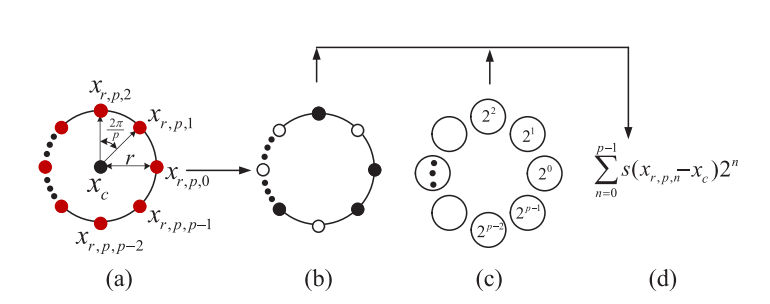
\includegraphics[width= 1\linewidth]{figures/lbp_oper.png}
	\caption{Hoạt động của LBP với bán kính r và p điểm ảnh xung quanh \cite{Liu2016}}
	\label{fig:lbp_oper}
\end{figure} 

Với $s()$ là hàm dấu (sign function). Nếu tọa độ của $x_c$ là (0, 0) thì tọa độ của các điểm xung quanh $x_{p, r, n}$ là $(-rsin(2\pi n/p), rcos(2\pi n /p))$. Giá trị của $x_{p,r,n}$ có thể không là giá trị ở vị trí trung tâm mà có thể sẽ được ước tính bằng phương pháp nội suy.
\begin{figure} [h]
	\centering
	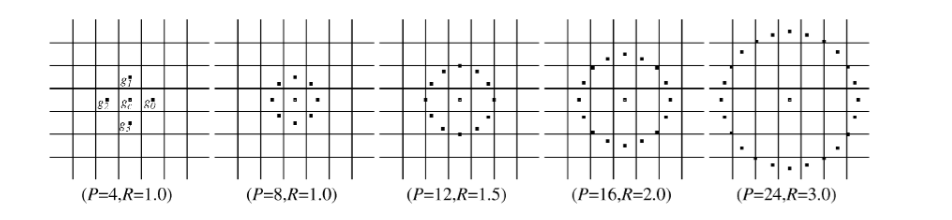
\includegraphics[width= 1\linewidth]{figures/lbpCircularSymmetric.png}
	\caption{LBP với các mẫu bán kính và điểm ảnh lân cận\cite{Ojala}}
	\label{fig:lbpCircularSymmetric}
\end{figure} 
Tuy nhiên, LBP vẫn bị ảnh hưởng nhiều bởi yếu tố độ xoay. Để giảm thiểu sự ảnh hưởng này, một biến thể LBP khác được đưa ra để đạt được sự bất biến của độ quay. Với p giá trị điểm ảnh lân cận, dựa vào toán tử LBP có thể có $2^p$ giá trị đầu ra khác nhau. Khi ảnh được xoay, giá trị nhị phân có được ở vị trí thứ x sẽ di chuyển xung quanh giá trị trung tâm. Do đó, để giảm sự ảnh hưởng của sự quay, Ojala \cite{Ojala} đã định nghĩa ra một định nghĩa như sau:

\begin{equation}
	LBP_{r, p}^{ri} = min\{ROR(LBP_{r, p}i) |  i = 0, 1, 2, ..., P-1\}
\end{equation}

Với $ROR(x, i)$ thực hiện việc dịch bit sang phải theo hình tròn. Với p điểm ảnh xung quanh, thì ta sẽ cần dịch đi i lần. Có thể hiểu đơn giản là ta sẽ đi tìm giá trị nhỏ nhất của một dãy bit bằng cách dịch chúng. Ví dụ với 8 điểm ảnh xung quanh, với dãy bit là $10000000_2$, ta có thể có rất nhiều giá trị như $01000000_2$ ứng với $64_{10}$ hay $00000001_2$ ứng với $1_{10}$. Nhưng khi thực hiện toàn bộ phép dịch và lấy giá trị nhỏ nhất, ta có thể đạt được giá trị là $1_{10}$, và đây là giá trị duy nhất. Các điểm ảnh khác nếu có thể đạt được giá trị như $00010000_2$, sau đó cũng được chuyển thành giá trị $1_{10}$ ở hệ thập phân. Hình \ref{fig:lbpRotation} mô tả số giá trị đặc trưng có thể có với p = 8. Mẫu số 0 giúp nhận biết điểm sáng, số 8 giúp nhận biết điểm tối, mẫu số 4 giúp nhận biết biên.  


\begin{figure} [h]
	\centering
	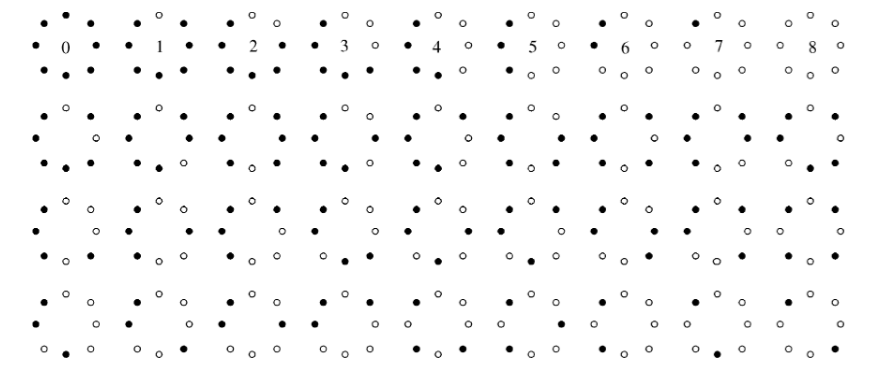
\includegraphics[width= 1\linewidth]{figures/lbpRotation.png}
	\caption{36 giá trị đặc trưng ứng với 8 giá trị điểm ảnh lân cận \cite{Ojala}}
	\label{fig:lbpRotation}
\end{figure} 

Để cải thiện thêm về tính bất biến của độ xoay, một khái niệm được đưa ra là \textbf{đồng nhất (uniform)}. Một mẫu đồng nhất sẽ chứa ít sự thay đổi về mặt không gian. Chúng hoạt động như các khuôn mẫu cho các cấu trúc vi mô như điểm sáng (0), vùng tối (8) hoặc các cạnh có độ cong âm hay dương (1-7). Để định nghĩa một mẫu là đồng nhất, Ojala giới thiệu một phương pháp gọi là U("pattern"), chúng chỉ đo lường sự thay đổi về mặt không gian (tức là sự thay đổi các bit từ 0 thành 1 hay từ 1 thành 0). Ví dụ, mẫu $00000000_2$ và mẫu $11111111_2$ có giá trị U bằng 0, trong khi đó 7 giá trị khác ở dòng đầu ở hình \ref{fig:lbpRotation}
 có giá trị U bằng 2 vì có chính xác 2 lần thay đổi bit từ 0 thành 1 và từ 1 thành 0. Trong khi đó, 27 mẫu còn lại có giá trị U ít nhất là 4. Từ đó, ta có định nghĩa về LBP đồng nhất như sau (đặt ngưỡng giá trị của U tối đa là T):

 \begin{equation}
     LBP_{r, p}^{riuT} = 
     \begin{cases}
         \sum_{i=0}^{p-1}s(gi - gc)  & \text{nếu} \quad U(LBP) \leq T
         \\
         p+1 & \text{còn lại}
     \end{cases}
     \label{eq:riu2}
 \end{equation}
 Với
 \begin{equation}
     U(LBP_{r, p}) = | s(g_{p-1} - g_c) - s(g_0 -g_c)| + \sum_{i = 1}^{p-1}|s(g_i - g_c) - s(g_{i-1} - g_c)| 
 \end{equation}
 
\begin{figure} [h]
	\centering
	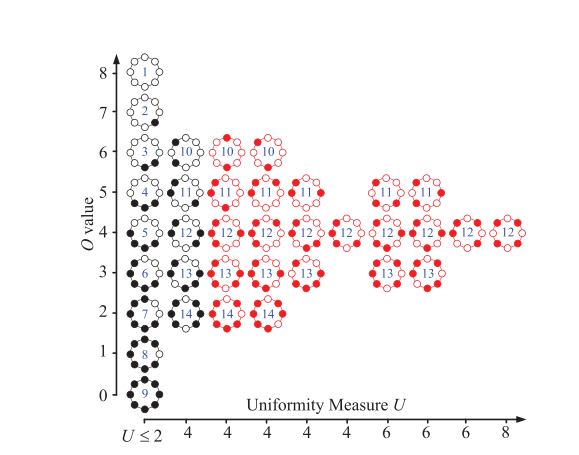
\includegraphics[width= 0.8\linewidth]{figures/lbpU.png}
	\caption{Số lượng các mẫu theo U với p = 8 \cite{Liu2016}}
	\label{fig:lbpU}
\end{figure} 

 Từ \textbf{riuT} thể hiện việc sử dụng mẫu đồng nhất với ngưỡng T và áp dụng việc dịch phải theo hình tròn. Nếu chỉ áp dụng mẫu đồng nhất T, ta có thể sử dụng từ \textbf{uT}. Ví dụ với T = 2, thì ta sẽ có phiên bản $LBP_{r, p}^{u2}$. Với p = 8, ta sẽ có tập hợp các mẫu ứng với giá trị của U, được mô tả trong hình \ref{fig:lbpU}.
\subsection{Các biến thể của LBP}
Có rất nhiều các biến thể của LBP đã được nghiên cứu nhằm mục đích tăng cường sự mạnh mẽ và khả năng phân biệt. Từ khảo sát từ Di Huang \cite{lbpVariantSurvey}, bảng \ref{tab:lbpVariant} mô tả một vài biến thể của LBP. 


\begin{table}[h]
    \centering
    \renewcommand{\arraystretch}{1.3} % Tăng khoảng cách dòng
        \caption{Một vài biến thể của LBP}
    \begin{tabular}{p{4cm} p{7cm} p{3cm}}
        \toprule
        \textbf{Tên biến thể} & \textbf{Đặc điểm} & \textbf{Mục tiêu} \\
        \midrule
        Extended LBP & Sử dụng thêm một số đơn vị nhị phân bổ sung  & Nâng cao khả năng phân biệt
        \\ \midrule
        Completed LBP & Xem xét cả dấu và độ lớn của các mẫu cục bộ & Nâng cao khả năng phân biệt
        \\ \midrule
        Soft LBP & Kết hợp các thành viên trong việc biểu diễn các mẫu cục bộ & Tăng cường khả năng chống nhiễu
        \\ \midrule 
        Local Tenary Binary & Sử dụng ngưỡng để tạo sự khác biệt & Tăng cường khả năng chống nhiễu
        \\
                   \bottomrule

    \end{tabular}

    \label{tab:lbpVariant}
\end{table}



\newpage
\subsection{Median Robust Extended Local Binary Pattern}

\begin{figure} [h]
	\centering
	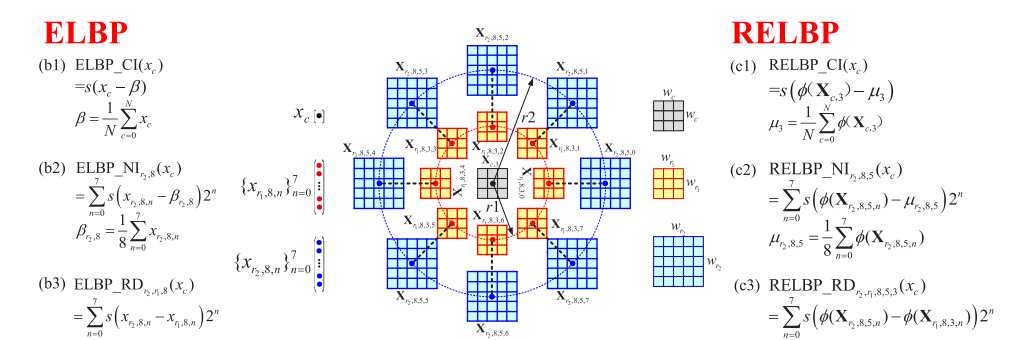
\includegraphics[width= 1\linewidth]{figures/elbpARelbp.png}
	\caption{Sự khác nhau giữa trích xuất đặc trưng của ELBP và RELBP \cite{Liu2016}}
	\label{fig:elbpARelbp}
\end{figure} 
Với ELBP, một trong những khuyết điểm của nó là bị ánh hưởng nhiều bởi nhiễu, do đó cần phải thay thế cường độ pixel riêng lẻ tại một điểm bằng một số biểu diễn trên một vùng. Các phương pháp đáng chú ý theo hướng này bao gồm BRIEF, BRISK và FREAK, trong đó trong mọi trường hợp, một vector mô tả nhị phân được tính bằng cách so sánh cường độ của một số cặp pixel sau khi áp dụng làm mịn Gaussian để làm giảm độ nhiễu. Li Liu \cite{Liu2016} xem xét tác động của việc thay thế các giá trị độ xám riêng lẻ tại các điểm lấy mẫu bằng cách dùng các bộ lọc đơn giản từ ảnh gốc và các vùng trong ảnh gốc. Đặc trưng của ELBP được thay đổi từ cường độ pixel tại các điểm riêng lẻ được thay thế bằng phản hồi từ các bộ lọc $\phi()$. Hình \ref{fig:elbpARelbp} thể hiện sự khác nhau giữa 2 phiên bản. Từ đó, định nghĩa ra Robust Extended Local Binary Pattern (RELBP) với các mô tả như sau:

\begin{enumerate}
    \item Biểu diễn điểm ảnh trung tâm 
    \begin{equation}
        RELBP\_CI(x_c) = s(\phi(\mathbf{X}_{c, w}) - \mu_w)
         \label{eq:relbp_ci}
    \end{equation}
    $\begin{cases}
    \phi(\mathbf{X}_{c,w}) \text{ là kết quả sau khi áp dụng bộ lọc lên điểm ảnh } X, \\
    \text{Vùng cục bộ có kích thước } w \times w \text{ ở xung quanh vị trí điểm ảnh trung tâm}, \\
    \mu_w \text{ kí hiệu cho giá trị trung bình của } \phi(X_{c,w}) \text{ trong toàn bộ bức ảnh}.
\end{cases}$



    \item Biểu diễn các giá trị lân cận
\begin{equation}
    \begin{aligned}
        RELBP\_NI_{r, p}(x_c) &= \sum_{n=0}^{p-1}s(\phi(\mathbf{X}_{r, p, w_r, n}) - \mu_{r, p, w_r}) 2^n \\
        \mu_{r, p, w_r} &= \frac{1}{p}\sum_{n =0}^{p-1}\phi(\mathbf{X}_{r, p, w_r, n})
    \end{aligned}
             \label{eq:relbp_ni}
\end{equation}

    \item Biểu diễn chênh lệch hướng tâm
    \begin{equation}
        RELBP\_RD_{r, r-1, p, w_r, w_{r-1}}(x_c) = \sum_{n=0}^{p-1}s(\phi(\mathbf{X}_{r, p, w_r, n}) - \phi(\mathbf{X}_{r-1, p, w_{r-1}, n}))2^n
             \label{eq:relbp_rd}
\end{equation}
\end{enumerate}

Các công thức \ref{eq:relbp_ci}, \ref{eq:relbp_ni}, \ref{eq:relbp_rd} là cách thực hiện tính toán đặc trưng với các thông tin có trong ảnh. Median Robust Extended Local Binary Pattern là phiên bản RELBP với bộ lọc được sử dụng là median. Phương pháp này có ưu điểm so với LBP truyền thống là mạnh hơn trước nhiễu và sự thay đổi của ảnh sáng. Nó nắm bắt thông tin kết cấu và thông tin không gian tốt hơn thông qua bộ lọc trung vị và mở rộng mẫu bên trong ảnh. Tuy vậy, MRELBP vẫn tồn tại một số nhược điểm như bị giới hạn ở các mẫu cục bộ. Tuy đã được mở rộng nhưng các kỹ thuật LBP vẫn tập trung vào các chi tiết cục bộ mà có thể bỏ sót các thay đổi ở kết cấu quy mô lớn. Kích thước bán kính cố định cũng là một nhược điểm, làm nó thiếu đi tính linh hoạt ở nhiều tỷ lệ khác nhau.

\section{Kiến trúc xử lý và giao tiếp dữ liệu}
\subsection{Pipelining}
Kỹ thuật đường ống (Pipelining) là một kỹ thuật được sử dụng trong các mạch số đồng bộ để tăng tần số hoạt động tối đa. Kỹ thuật này liên quan đến việc chèn thêm các thanh ghi ở các đường dẫn quan trọng, làm giảm số lượng logic giữa mỗi thanh ghi. Ít logic hơn sẽ tiêu tốn ít thời gian để thực hiện hơn, từ đó gia tăng tần số hoạt động tối đa.

Đường dẫn quan trọng (critical path) trong mạch là đường dẫn giữa 2 thanh ghi liên tiếp với độ trễ cao nhất. Điều đó cũng tương đương với việc thời gian để có giá trị đầu ra giữa 2 thanh ghi này là lâu nhất.  Hình \ref{fig:pipeline1} mô tả mạch trước khi được pipelining. Trong đó, thời gian thực hiện 2 mạch tổ hợp giữa 2 thanh ghi là thời gian của mạch A cộng với mạch B. Do đó, thời gian tính toán tổ hợp tốn 20ms. Ở hình \ref{fig:pipeline2} đã thực hiện pipelining bằng cách chèn vào giữa A và B một thanh ghi, do đó thời gian tối đa trong tính toán tổ hợp chỉ là 15ms. Do đó, kĩ thuật pipelining sẽ giúp tăng lên tần số hoạt động tối đa của mạch. 
\begin{figure}[!ht]
    \centering
    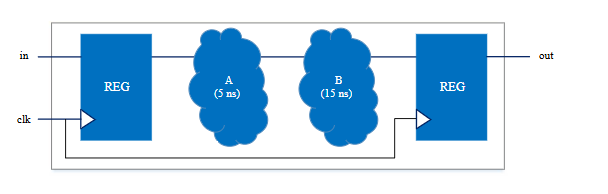
\includegraphics[width=\linewidth]{figures/pipeline1.png}
    \caption{Mạch trước khi pipelining}
    \label{fig:pipeline1}
\end{figure}
\begin{figure}[!ht]
    \centering
    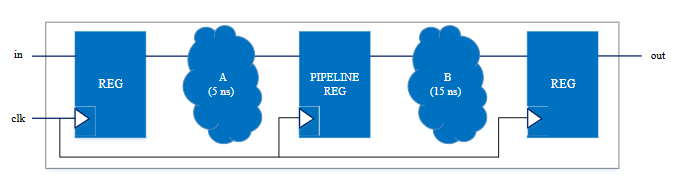
\includegraphics[width=\linewidth]{figures/pipeline2.png}
    \caption{Mạch sau khi pipelining}
    \label{fig:pipeline2}
\end{figure}
\subsection{Giao diện AXI4-Stream}
Trong một hệ thống System on Chip (SoC), BUS là thành phần chính kết nối các thiết bị chính và thiết bị phụ. Nó giúp các thiết bị chính có thể truy xuất (đọc/ghi) các slave bằng cách chuyển thông tin điều khiển từ thiết bị chính đến thiết bị phụ, đồng thời chuyển dữ liệu và thông tin phản hồi từ thiết bị phụ đến thiết bị chính. AXI (Advanced eXtensible Interface) là một trong các giao thức BUS trong họ AMBA (Advanced Microcontroller Bus Architecture), được phát triển bởi hãng ARM. 

AXI4-Stream là một liên kết điểm tới điểm, bên gửi là thiết bị chính còn bên nhận là thiết bị phụ. Để giao tiếp được giữa hai bên, cần một quá trình gọi là bắt tay. Hình \ref{fig:axi4} mô tả quá trình truyền dữ liệu đối với kênh AXI4-Stream. Tín hiệu \textbf{tvalid} được phát bởi bên truyền và \textbf{tready} được phát bởi bên nhận. Tín hiệu \textbf{tvalid} chỉ ra rằng dữ liệu \textbf{tdata} là hợp lệ. Tín hiệu \textbf{tready} chỉ ra rằng bên nhận sẵn sàng để nhận dữ liệu. Khi mà cả \textbf{tvalid} và \textbf{tready} đều ở mức cao thì quá trình truyền diễn ra.


\begin{figure}[!ht]
    \centering
    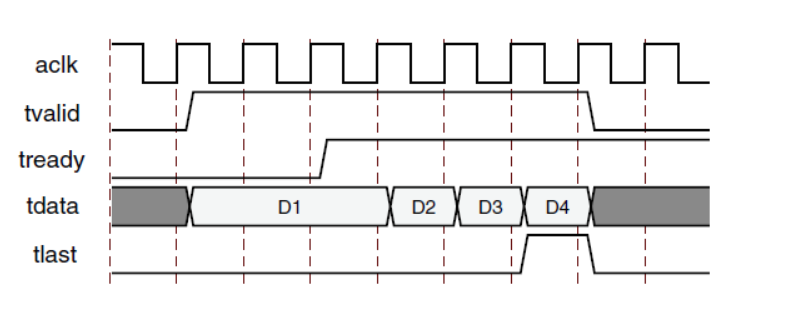
\includegraphics[width=\linewidth]{figures/axi4.png}
    \caption{Truyền dữ liệu ở kênh AXI4-Stream}
    \label{fig:axi4}
\end{figure}
\section{Phần mềm thiết kế và mô phỏng Vivado}
\begin{figure}[!ht]
	\centering
	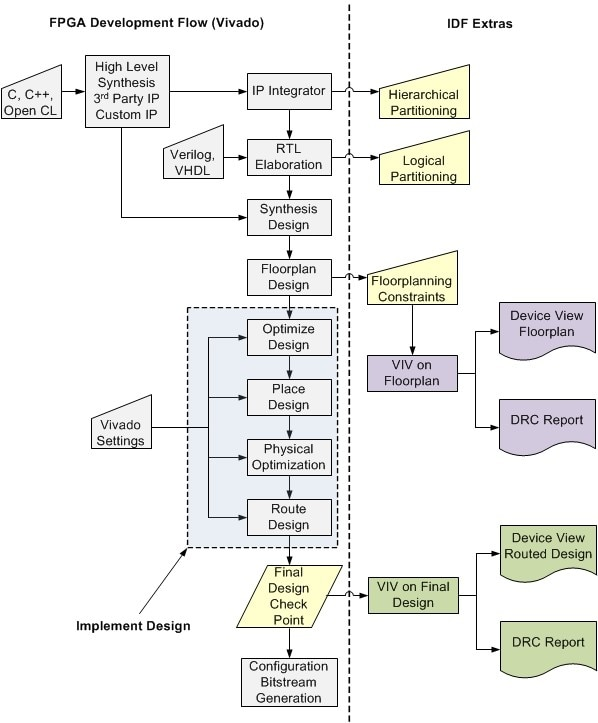
\includegraphics[width=\linewidth]{figures/3311000-fpga-development-flow.jpg}
	\caption{Chu trình thiết kế và tổng hợp của Vivado}
	\label{fig:fpga_dev}
\end{figure}


Vivado Design Suite là một tổ hợp các phần mềm của hãng Xilinx để tổng hợp và phân tích các thiết kế từ ngôn ngữ mô tả phần cứng. Trình mô phỏng Vivado là một thành phần của Vivado Design Suite, dùng để mô phỏng với các ngôn ngữ mô tả phần cứng được biên dịch, trong đó hỗ trợ tập lệnh TCL, IP đã thiết kế và xác minh nâng cao. Hình \ref{fig:fpga_dev} mô tả chu trình phát triển FPGA sử dụng phần mềm Xilinx Vivado. Đối với các phương pháp tổng hợp mức cao, mô-đun sẽ được thiết kế sử dụng những ngôn ngữ bậc cao như C, C++... Thông qua các trình tổng hợp mức cao để có được những thiết kế có thể tổng hợp. Đối với phương pháp thiết kế ở mức RTL (Register Transfer Level), Vivado hỗ trợ các trình biên dịch có thể biên dịch với các ngôn ngữ mô tả phần cứng bao gồm SystemVerilog, Verilog và VHDL. Sau khi có thiết kế, có thể tiến hành tổng hợp tạo thành các các mạng lưới cổng logic (netlist) cụ thể cho thiết bị FPGA. Sau đó đến các quá trình thực thi (implementation) biến các thiết kế logic thành các bố trí cụ thể trên FPGA. Sau khi đã đảm bảo các yếu tố về thời gian, DRC (Design Rule Check) có thể tiến hành tạo ra các bitstream để cấu hình cho FPGA.
